\section{Σχεδιασμός Έλλειψης}

    Έστω ότι θέλουμε να σχεδιάσουμε έλλειψη με κέντρο το $O (0,0)$ και άξονες με διάμετρο $2a$ και $2b$, $a, b \in \mathbb{Z}$. Η έλλειψη χαρακτηρίζεται από 4πλή συμμετρία.

\begin{figure}[hbt]
  \begin{center}
	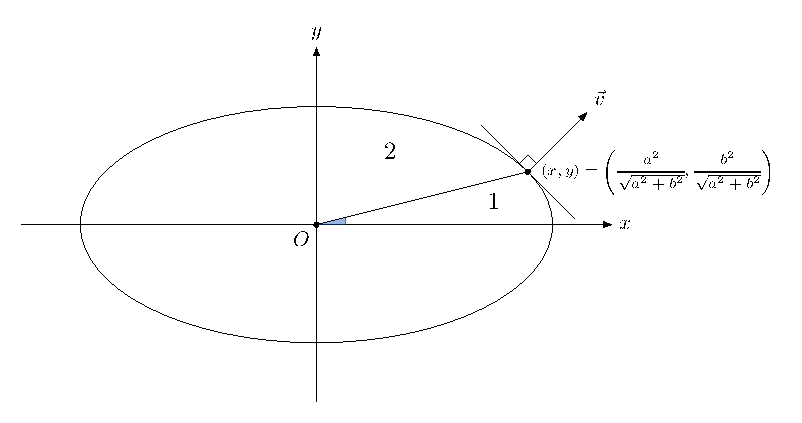
\includegraphics[scale=1]{Figures/Chapter1/Ellipse/figure1.pdf}
  \end{center}
  \caption{Έλλειψη}
\end{figure}

Ο διαχωρισμός σε περιοχή 1 και περιοχή 2 γίνεται εκεί όπου

\[
\frac{dy}{dx} = -1
\]
Εξίσωση Έλλειψης

\[
\frac{x^2}{a^2} + \frac{y^2}{b^2} = 1
\]

\[
f(x,y) = b^2x^2 + a^2y^2 - a^2b^2 = 0
\]
\subsection{Υπολογιστική Πολυπλοκότητα}

\begin{tabular}{m{0.2\textwidth}m{0.4\textwidth}}
	  Περιοχή 1: & \( y_r \) βήματα της \( y \)-κατεύθυνσης.\\
	& \( a - x_r \) βήματα της \( x \)-κατεύθυνσης.\\
	& Υπολογίζονται \( y_r \) σημεία.
\end{tabular}

\begin{tabular}{m{0.2\textwidth}m{0.4\textwidth}}
	Περιοχή 2: & \( x_r \) βήματα της \( x \)-κατεύθυνσης.\\
	& \( b - y_r \) βήματα της \( y \)-κατεύθυνσης.\\
	& Υπολογίζονται \( x_r \) σημεία.
\end{tabular}

Για \( (1) \) βήμα στην \( y \)-κατεύθυνση στην περιοχή 1 απαιτούνται 3 προσθέσεις (ανάλογα για τα βήματα της \( x \)-κατεύθυνσης της περιοχής 2) ανά σημείο κατά μέσο όρο:
\[
\frac{3y_r + 2(a-x_r) +3x_r + 2(b-y_r)}{ x_r +y_r} = 1+ 2\frac{a+b}{\sqrt{a^2 + b^2 }}, \text{ προσθέσεις, } \frac{a+b}{\sqrt{a^2 + b^2}} \text{ αυξήσεις ανά σημείο.}
\]

\begin{figure}[hbt]
  \begin{center}
	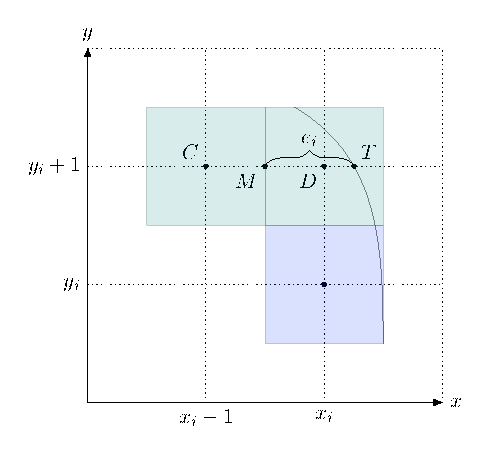
\includegraphics[scale=1]{Figures/Chapter1/Ellipse/figure2.pdf}
  \end{center}
  \caption{Περιοχή 1}
\end{figure}

\subsection*{Περιοχή 1:}
Έστω ότι έχει φωτισθεί το pixel $(x_i, y_i)$. Επειδή βρισκόμαστε στην περιοχή 1, το επόμενο προς φωτισμό pixel θα είναι το $(x_i, y_i+1)$ ή το $(x_i-1, y_i+1)$. Παρατηρούμε ότι αυξάνεται κατά 1 η $y$ συντεταγμένη και χρειαζόμαστε ένα κριτήριο.

Απόφαση για το αν θα φωτιστεί η $x_i$ ή $x_{i-1}$ θέση. Έστω $M$ το μέσο του ευθύγραμμου τμήματος $CD$. Οι συντεταγμένες του μέσου $M$ θα είναι

\begin{equation}
    f(M) = f \left( \frac{x_i + x_{i-1}}{2}, y_i + 1 \right) = f \left( x_i - \frac{1}{2}, y_i + 1 \right)
\end{equation}

Εάν $T$ είναι το σημείο τομής της έλλειψης με το ευθύγραμμο τμήμα $CD$ και $e_i$ η απόσταση από το μέσο $M$, τότε αυτό ικανοποιεί την εξίσωση της έλλειψης και θα ισχύει:

\begin{equation}
    f \left( x_i - \frac{1}{2} + e_1, y_i + 1 \right) = b^2 \left( x_i - \frac{1}{2} + e_1 \right)^2 + a^2 (y_i + 1)^2 - 4a^2b^2 = 0
\end{equation}

Αναπτύσσοντας την προηγούμενη έκφραση έχουμε ότι:

\begin{equation}
    f \left( x_i - \frac{1}{2}, y_i + 1 \right) = - \left( 2b^2 \left( x_i - \frac{1}{2} \right) e_1 + b^2 e_1^2 \right) = 0
\end{equation}

Εάν ονομάσουμε μεταβλητή απόφασης για την περιοχή 1, $f_{mid1}$ τις συντεταγμένες του μέσου $M$ θα έχουμε:

\begin{equation}
    f_{mid1} = f(M) = - \left( 2b^2 \left( x_i - \frac{1}{2} \right) e_1 + b^2 e_1^2 \right)
\end{equation}

Παρατηρούμε ότι το πρόσημο της έκφρασης του $f(M)$ καθορίζει την επιλογή του επόμενου σημείου. Συγκεκριμένα:

\begin{table}[htb]
    \centering
    \begin{tabular}{@{}c|c@{}}
        \toprule
        $f(M)$ & Επιλογή σημείου \\  \midrule
        $< 0$ & $e_1 > 0 \Rightarrow$ Το $T$ δεξιότερα του $M$, επιλογή του σημείου $D$ \\
        $\geq 0$ & $e_1 \leq 0 \Rightarrow$ Το $T$ αριστερότερα του $M$, επιλογή του σημείου $C$ \\
        \bottomrule
    \end{tabular}
\end{table}

\subsection{Αναδρομικός υπολογισμός των $f_{mid1}$ και $f_{mid2}$}

Είναι απαραίτητο να υπάρχει μια σχέση σύνδεσης ανάμεσα στις δύο μεταβλητές απόφασης. Έχουμε ότι Περιοχή 1:

\begin{equation}
    f_{mid1, i+1} = f(x_{i+1} - \frac{1}{2}, y_{i+1} + 1) = b^2 (x_{i+1} - \frac{1}{2}) + a^2(y_{i+1} + 1)^2 - a^2b^2
\end{equation}

Στην περιοχή 1 ισχύει ότι $y_{i+1} = y_i + 1$, έτσι προκύπτει:

\begin{table}[htb]
    \centering
    \begin{tabular}{@{}c|c@{}}
        \toprule
        $f_{mid1,i+1}$ & Επιλογή Σημείου \\
        \midrule
        $f_{mid1,i} + 2a^2 y_{i+1} + a^2$ & D \\
        $f_{mid1,i} + 2a^2 y_{i+1} + a^2 - 2b^2 x_{i+1}$ & C \\
        \bottomrule
    \end{tabular}
\end{table}

\subsection{Επιλογή αρχικής τιμής για την $f_{mid1}$}
Για $(x_1, y_1) = (a,0)$ προκύπτει ότι:

\begin{equation}
    f_{mid1,1} = f \left(x_1 - \frac{1}{2}, y_1 + 1 \right) = a^2 - b^2 a + \frac{b^2}{4}
\end{equation}
\begin{figure}[hbt]
  \begin{center}
	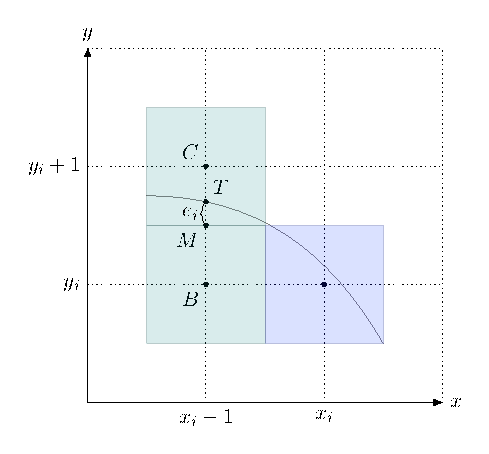
\includegraphics[scale=1]{Figures/Chapter1/Ellipse/figure3.pdf}
  \end{center}
  \caption{Περιοχή 2}
\end{figure}
Αντίστοιχη διαδικασία ισχύει και για την περιοχή 2. Συγκεκριμένα προκύπτει ότι:

\begin{table}[htb]
    \centering
    \begin{tabular}{@{}c|c@{}}
        \toprule
        $f_{mid2,i+1}$ & Επιλογή Σημείου \\
        \midrule
        $f_{mid2,i} - 2b^2 x_{i+1} + b^2$ & B \\
        $f_{mid2,i} - 2b^2 x_{i+1} + b^2 - 2a^2 x_{i+1}$ & D \\
        \bottomrule
    \end{tabular}
\end{table}

\subsection{Καθορισμός συνόρου μεταξύ της περιοχής 1 \& 2}

Επειδή η αλλαγή της περιοχής γίνεται στο σημείο όπου η κλίση της εφαπτομένης ισούται με -1 υπολογίζουμε την παράγωγο της εξίσωσης της έλλειψης:

\begin{equation}
    y^2 = b^2 - \frac{b^2}{a^2} x^2, \quad \frac{dy}{dx} = - \frac{2b^2 x}{2a^2 y}
\end{equation}

\begin{equation}
    \frac{dy}{dx} > -1 \Rightarrow 2a^2 y > 2b^2 x
\end{equation}

Όταν λοιπόν $2a^2 y > 2b^2 x$ έχουμε περάσει από την περιοχή 1 στην περιοχή 2. Για την ανάπτυξη του αλγορίθμου της έλλειψης θα ήταν επιθυμητό να χρησιμοποιήσουμε μόνο μια μεταβλητή απόφασης. Παρατηρούμε ότι η μετάβαση από το σύνορο μπορεί να υπολογισθεί με βάση την $f_{mid1}$. Συγκεκριμένα παρατηρούμε ότι:

\begin{equation}
    f_{mid2} - f_{mid1} = \left( b^2 x_i + a^2 y_i \right) + \frac{3}{4} \left( b^2 - a^2 \right)
\end{equation}

Τελικά

\begin{equation}
    f_{mid2} = f_{mid1} - \frac{2b^2 x_i + 2a^2 y_i}{2} + 0.75 \left( b^2 - a^2 \right)
\end{equation}

\begin{lstlisting}[caption={Γενικός αλγόριθμος σχερδιασμού ελλειψής του Bresenham }]
function elipsis(a, b, color)
    hold on
    x = a;
    y = 0;
    asqr = a^2;
    bsqr = b^2;
    a22 = 2 * asqr;
    b22 = 2 * bsqr;
    xslope = b22 * a;
    yslope = 0;
    fmid = bsqr * (0.25 - x) + asqr;

    % Area 1
    while (xslope > yslope)
        image(x, y, color)
        image(-x, -y, color)
        image(x, -y, color)
        image(-x, y, color)
        y = y + 1;
        yslope = yslope + a22;

        if fmid >= 0
            x = x - 1;
            xslope = xslope - b22;
            fmid = fmid - xslope;
        end
        fmid = fmid + yslope + asqr;
    end

    % Border correction
    fmid = fmid - (yslope + xslope)/2 + 0.75 * (bsqr - asqr);

    % Area 2
    while (x > 0)
        image(x, y, color)
        image(-x, -y, color)
        image(x, -y, color)
        image(-x, y, color)
        x = x - 1;
        xslope = xslope - b22;

        if fmid <= 0
            y = y + 1;
            yslope = yslope + a22;
            fmid = fmid + yslope;
        end
        fmid = fmid - xslope + bsqr;
    end
endfunction
\end{lstlisting}